% Options for packages loaded elsewhere
% Options for packages loaded elsewhere
\PassOptionsToPackage{unicode}{hyperref}
\PassOptionsToPackage{hyphens}{url}
\PassOptionsToPackage{dvipsnames,svgnames,x11names}{xcolor}
%
\documentclass[
  letterpaper,
  DIV=11,
  numbers=noendperiod]{scrartcl}
\usepackage{xcolor}
\usepackage{amsmath,amssymb}
\setcounter{secnumdepth}{-\maxdimen} % remove section numbering
\usepackage{iftex}
\ifPDFTeX
  \usepackage[T1]{fontenc}
  \usepackage[utf8]{inputenc}
  \usepackage{textcomp} % provide euro and other symbols
\else % if luatex or xetex
  \usepackage{unicode-math} % this also loads fontspec
  \defaultfontfeatures{Scale=MatchLowercase}
  \defaultfontfeatures[\rmfamily]{Ligatures=TeX,Scale=1}
\fi
\usepackage{lmodern}
\ifPDFTeX\else
  % xetex/luatex font selection
\fi
% Use upquote if available, for straight quotes in verbatim environments
\IfFileExists{upquote.sty}{\usepackage{upquote}}{}
\IfFileExists{microtype.sty}{% use microtype if available
  \usepackage[]{microtype}
  \UseMicrotypeSet[protrusion]{basicmath} % disable protrusion for tt fonts
}{}
\makeatletter
\@ifundefined{KOMAClassName}{% if non-KOMA class
  \IfFileExists{parskip.sty}{%
    \usepackage{parskip}
  }{% else
    \setlength{\parindent}{0pt}
    \setlength{\parskip}{6pt plus 2pt minus 1pt}}
}{% if KOMA class
  \KOMAoptions{parskip=half}}
\makeatother
% Make \paragraph and \subparagraph free-standing
\makeatletter
\ifx\paragraph\undefined\else
  \let\oldparagraph\paragraph
  \renewcommand{\paragraph}{
    \@ifstar
      \xxxParagraphStar
      \xxxParagraphNoStar
  }
  \newcommand{\xxxParagraphStar}[1]{\oldparagraph*{#1}\mbox{}}
  \newcommand{\xxxParagraphNoStar}[1]{\oldparagraph{#1}\mbox{}}
\fi
\ifx\subparagraph\undefined\else
  \let\oldsubparagraph\subparagraph
  \renewcommand{\subparagraph}{
    \@ifstar
      \xxxSubParagraphStar
      \xxxSubParagraphNoStar
  }
  \newcommand{\xxxSubParagraphStar}[1]{\oldsubparagraph*{#1}\mbox{}}
  \newcommand{\xxxSubParagraphNoStar}[1]{\oldsubparagraph{#1}\mbox{}}
\fi
\makeatother


\usepackage{longtable,booktabs,array}
\newcounter{none} % for unnumbered tables
\usepackage{calc} % for calculating minipage widths
% Correct order of tables after \paragraph or \subparagraph
\usepackage{etoolbox}
\makeatletter
\patchcmd\longtable{\par}{\if@noskipsec\mbox{}\fi\par}{}{}
\makeatother
% Allow footnotes in longtable head/foot
\IfFileExists{footnotehyper.sty}{\usepackage{footnotehyper}}{\usepackage{footnote}}
\makesavenoteenv{longtable}
\usepackage{graphicx}
\makeatletter
\newsavebox\pandoc@box
\newcommand*\pandocbounded[1]{% scales image to fit in text height/width
  \sbox\pandoc@box{#1}%
  \Gscale@div\@tempa{\textheight}{\dimexpr\ht\pandoc@box+\dp\pandoc@box\relax}%
  \Gscale@div\@tempb{\linewidth}{\wd\pandoc@box}%
  \ifdim\@tempb\p@<\@tempa\p@\let\@tempa\@tempb\fi% select the smaller of both
  \ifdim\@tempa\p@<\p@\scalebox{\@tempa}{\usebox\pandoc@box}%
  \else\usebox{\pandoc@box}%
  \fi%
}
% Set default figure placement to htbp
\def\fps@figure{htbp}
\makeatother





\setlength{\emergencystretch}{3em} % prevent overfull lines

\providecommand{\tightlist}{%
  \setlength{\itemsep}{0pt}\setlength{\parskip}{0pt}}



 


\KOMAoption{captions}{tableheading}
\makeatletter
\@ifpackageloaded{caption}{}{\usepackage{caption}}
\AtBeginDocument{%
\ifdefined\contentsname
  \renewcommand*\contentsname{Table of contents}
\else
  \newcommand\contentsname{Table of contents}
\fi
\ifdefined\listfigurename
  \renewcommand*\listfigurename{List of Figures}
\else
  \newcommand\listfigurename{List of Figures}
\fi
\ifdefined\listtablename
  \renewcommand*\listtablename{List of Tables}
\else
  \newcommand\listtablename{List of Tables}
\fi
\ifdefined\figurename
  \renewcommand*\figurename{Figure}
\else
  \newcommand\figurename{Figure}
\fi
\ifdefined\tablename
  \renewcommand*\tablename{Table}
\else
  \newcommand\tablename{Table}
\fi
}
\@ifpackageloaded{float}{}{\usepackage{float}}
\floatstyle{ruled}
\@ifundefined{c@chapter}{\newfloat{codelisting}{h}{lop}}{\newfloat{codelisting}{h}{lop}[chapter]}
\floatname{codelisting}{Listing}
\newcommand*\listoflistings{\listof{codelisting}{List of Listings}}
\makeatother
\makeatletter
\makeatother
\makeatletter
\@ifpackageloaded{caption}{}{\usepackage{caption}}
\@ifpackageloaded{subcaption}{}{\usepackage{subcaption}}
\makeatother
\usepackage{bookmark}
\IfFileExists{xurl.sty}{\usepackage{xurl}}{} % add URL line breaks if available
\urlstyle{same}
\hypersetup{
  pdftitle={Guia Practica},
  pdfauthor={Universidad Nacional de Cordoba. FCE},
  colorlinks=true,
  linkcolor={blue},
  filecolor={Maroon},
  citecolor={Blue},
  urlcolor={Blue},
  pdfcreator={LaTeX via pandoc}}


\title{Guia Practica}
\usepackage{etoolbox}
\makeatletter
\providecommand{\subtitle}[1]{% add subtitle to \maketitle
  \apptocmd{\@title}{\par {\large #1 \par}}{}{}
}
\makeatother
\subtitle{Economia Politica}
\author{Universidad Nacional de Cordoba. FCE}
\date{}
\begin{document}
\maketitle


\newpage

\subsection{Presentacion}\label{presentacion}

\newpage

\section{Indice}\label{indice}

\begin{itemize}
\item
  \hyperref[1]{Unidad 1}
\item
  \hyperref[2]{Unidad 2}

  \begin{itemize}
  \tightlist
  \item
    \hyperref[2_1]{Sistemas de Votación}
  \item
    \hyperref[2_2]{Modelo de Meltzer \& Richard}
  \item
    \hyperref[2_3]{Pico Único y Cruce Único}
  \end{itemize}
\item
  \hyperref[3]{Unidad 3}

  \begin{itemize}
  \tightlist
  \item
    \hyperref[3_1]{Modelo simple de no democracia}
  \item
    \hyperref[3_2]{Modelo Democratización}
  \end{itemize}
\item
  \hyperref[4]{Unidad 4}
\end{itemize}

\newpage

\section{Unidad 1}\label{1}

\newpage

\section{Unidad 2}\label{2}

\subsection{Sistemas de Votación}\label{2_1}

1.1) Suponga que existen 5 grupos de individuos con los siguientes
ordenamientos de preferencias sobre 5 alternativas

\begin{itemize}
\tightlist
\item
  Preferencias

  \begin{itemize}
  \tightlist
  \item
    (21 personas) \(C>A>E>B>D\)
  \item
    (15 personas) \(B>D>A>C>E\)
  \item
    (12 personas) \(A>B>E>D>C\)
  \item
    (8 personas) \(D>C>E>A>B\)
  \item
    (4 personas) \(E>A>D>B>C\)
  \end{itemize}
\end{itemize}

Responda que alternativa resulta ganadora bajo los siguientes métodos de
votación colectiva:

\begin{enumerate}
\def\labelenumi{\alph{enumi})}
\tightlist
\item
  Pluralidad
\item
  Mayoría Absoluta
\item
  Votación de Condorcet
\item
  Método Borda (criterio de n-1)
\end{enumerate}

Respuestas:

\begin{enumerate}
\def\labelenumi{\alph{enumi})}
\tightlist
\item
  C
\item
  No hay ganador
\item
  A
\item
  A
\end{enumerate}

1.2) Suponga que existen 3 grupos de individuos con los siguientes
ordenamientos de preferencias sobre 5 alternativas

\begin{itemize}
\tightlist
\item
  Preferencias

  \begin{itemize}
  \tightlist
  \item
    (20 personas) \(A>C>D>B>E\)
  \item
    (13 personas) \(C>E>A>D>B\)
  \item
    (11 personas) \(E>B>D>A>C\)
  \end{itemize}
\end{itemize}

Responda que alternativa resulta ganadora bajo los siguientes métodos de
votación colectiva:

\begin{enumerate}
\def\labelenumi{\alph{enumi})}
\tightlist
\item
  Pluralidad
\item
  Mayoría Absoluta
\item
  Votación de Condorcet
\item
  Método Borda (criterio de n)
\end{enumerate}

Respuestas:

\begin{enumerate}
\def\labelenumi{\alph{enumi})}
\tightlist
\item
  A
\item
  No hay ganador
\item
  No hay ganador de Condorcet
\item
  A
\end{enumerate}

\hfill\break

\begin{enumerate}
\def\labelenumi{\arabic{enumi})}
\setcounter{enumi}{1}
\tightlist
\item
  Una elección acerca del siguiente ganador del Balón de Oro en octubre
  del 2024 debe ser decidida a través del método Borda. A la recta final
  llegaron 5 candidatos (A, B, C, D y E) y hay 45 votantes entre los
  cuales se encuentran grandes eminencias del deporte.
\end{enumerate}

Si el jugador A obtiene 136 puntos, el jugador B obtiene 129 puntos, el
C obtiene 148. el D obtiene 118 y E obtiene \textbf{?}.

¿Qué criterio se utiliza, ``n'' o ``n-1''? ¿Qué candidato será el
ganador del premio? ¿Cuántos votos obtuvo E?

\hfill\break

\begin{enumerate}
\def\labelenumi{\arabic{enumi})}
\setcounter{enumi}{2}
\tightlist
\item
  Condorcet: Se realizó una votación entre expertos del mundo del tenis
  para determinar quién fue el mejor tenista del ``Big Four'' al que
  componen Murray (M), Federer (F), Nadal (N) y Djokovic (D). Las
  preferencias de lo expertos son las siguientes:
\end{enumerate}

\begin{itemize}
\tightlist
\item
  (23 personas) \(F>D>N>M\)
\item
  (31 personas) \(D>N>F>M\)
\item
  (27 personas) \(N>F>D>M\)
\end{itemize}

Se resuelve una votacion de a pares. ¿Existe el ganador de Condorcet?

Respuesta: Hay Ciclo de Condorcet ya que las preferencias no son de pico
único.

\hfill\break

\begin{enumerate}
\def\labelenumi{\arabic{enumi})}
\setcounter{enumi}{3}
\item ~
  \subsubsection{Ejercicio 3: Condorcet}\label{ejercicio-3-condorcet}
\end{enumerate}

Se realizó una votación entre expertos del mundo del tenis para
determinar quién fue el mejor tenista del ``Big Four'', compuesto por
Murray (M), Federer (F), Nadal (N) y Djokovic (D). Las preferencias de
los expertos son las siguientes:

\begin{itemize}
\tightlist
\item
  \textbf{(23 personas):} \(F \succ D \succ N \succ M\)
\item
  \textbf{(31 personas):} \(D \succ N \succ F \succ M\)
\item
  \textbf{(27 personas):} \(N \succ F \succ D \succ M\)
\end{itemize}

Se resuelve mediante una votación de a pares. ¿Existe un ganador de
Condorcet?

\textbf{Respuesta:} Hay un \textbf{Ciclo de Condorcet}, ya que las
preferencias no son de pico único.

\begin{center}\rule{0.5\linewidth}{0.5pt}\end{center}

\subsubsection{Ejercicio 4: Sistemas de
Votación}\label{ejercicio-4-sistemas-de-votaciuxf3n}

Suponga que existen 5 grupos de individuos con los siguientes
ordenamientos de preferencias sobre 5 alternativas (A, B, C, D, E):

\begin{itemize}
\tightlist
\item
  \textbf{Grupo 1} (20 personas): \(B \succ D \succ C \succ A \succ E\)
\item
  \textbf{Grupo 2} (8 personas): \(B \succ C \succ D \succ E \succ A\)
\item
  \textbf{Grupo 3} (10 personas): \(C \succ A \succ D \succ B \succ E\)
\item
  \textbf{Grupo 4} (7 personas): \(A \succ C \succ D \succ E \succ B\)
\item
  \textbf{Grupo 5} (5 personas): \(D \succ C \succ A \succ B \succ E\)
\end{itemize}

¿Qué alternativa resulta ganadora bajo los siguientes sistemas de
votación: Pluralidad, Mayoría Absoluta, Condorcet y Método de Borda
(criterio n-1)? ¿Qué conclusiones obtiene después de observar los
distintos resultados?

\textbf{Respuesta:}

Teniendo en cuenta que hay 50 personas en total (20 + 8 + 10 + 7 + 5 =
50), la alternativa ganadora bajo cada uno de los criterios es:

\begin{enumerate}
\def\labelenumi{\arabic{enumi}.}
\item
  \textbf{Pluralidad:} Gana la alternativa \textbf{B} por tener la mayor
  cantidad de primeros lugares (28 votos en total: 20 del Grupo 1 + 8
  del Grupo 2).
\item
  \textbf{Mayoría Absoluta:} Para ganar, se requieren al menos 26 votos
  (la mitad más uno). Esta condición la cumple únicamente la alternativa
  \textbf{B} con sus 28 votos.
\item
  \textbf{Condorcet:} Realizamos los enfrentamientos de a pares
  empezando por la A:

  \begin{itemize}
  \tightlist
  \item
    \textbf{A vs B:} 22 vs 28 \(\rightarrow\) Gana \textbf{B} (A queda
    eliminada).
  \item
    \textbf{B vs C:} 28 vs 22 \(\rightarrow\) Gana \textbf{B}.
  \item
    \textbf{B vs D:} 28 vs 22 \(\rightarrow\) Gana \textbf{B}.
  \item
    \textbf{B vs E:} 43 vs 7 \(\rightarrow\) Gana \textbf{B}. La
    alternativa \textbf{B} gana todos sus enfrentamientos, por lo que es
    la ganadora de Condorcet.
  \end{itemize}
\item
  \textbf{Método de Borda (criterio n-1):} Asignamos puntajes del 4 al 0
  (donde el primer lugar vale 4 puntos, el segundo 3, etc.) y
  multiplicamos por la cantidad de personas en cada grupo:

  \begin{itemize}
  \tightlist
  \item
    \(A = (20 \cdot 1) + (8 \cdot 0) + (10 \cdot 3) + (7 \cdot 4) + (5 \cdot 2) = 88\)
  \item
    \(B = (20 \cdot 4) + (8 \cdot 4) + (10 \cdot 1) + (7 \cdot 0) + (5 \cdot 1) = 127\)
  \item
    \(C = (20 \cdot 2) + (8 \cdot 3) + (10 \cdot 4) + (7 \cdot 3) + (5 \cdot 3) = \textbf{140}\)
  \item
    \(D = (20 \cdot 3) + (8 \cdot 2) + (10 \cdot 2) + (7 \cdot 2) + (5 \cdot 4) = 130\)
  \item
    \(E = (20 \cdot 0) + (8 \cdot 1) + (10 \cdot 0) + (7 \cdot 1) + (5 \cdot 0) = 15\)
  \end{itemize}

  La alternativa \textbf{C} resulta ganadora con 140 puntos.
\end{enumerate}

\textbf{Conclusión:} En este perfil, la alternativa B gana casi todo en
votos directos (Pluralidad, Mayoría y Condorcet), pero C gana por el
método de Borda. Esto demuestra cómo distintos métodos de votación
pueden producir diferentes vencedores.

También evidencia que puede existir un ganador de Condorcet (B) que no
coincida con el ganador del método de Borda (C). Además, dado que C gana
por Borda siendo la favorita \emph{únicamente} del Grupo 3, se muestra
que puede resultar ganadora una alternativa que no sea la favorita
general (o de varios grupos), pero que está consistentemente bien
rankeada (segunda o tercera opción) entre todos los votantes.

\hfill\break

\begin{enumerate}
\def\labelenumi{\arabic{enumi})}
\setcounter{enumi}{4}
\item ~
  \subsubsection{Ejercicio: Votación de The
  Beatles}\label{ejercicio-votaciuxf3n-de-the-beatles}
\end{enumerate}

Los miembros del comité editorial de la revista Rolling Stone se
reunieron para votar cuál fue el mejor integrante de los Beatles con el
fin de decidir a quién dedicar el próximo número de la revista. La
comisión estaba formada por 60 expertos, quienes expresaron sus
preferencias completas sobre los cuatro Beatles: Ringo (R), George (G),
John (J) y Paul (P). El resultado de las votaciones fue el siguiente:

\begin{itemize}
\tightlist
\item
  \textbf{Grupo 1} (20 expertos): \(R \succ P \succ G \succ J\)
\item
  \textbf{Grupo 2} (18 expertos): \(P \succ G \succ J \succ R\)
\item
  \textbf{Grupo 3} (22 expertos): \(G \succ J \succ R \succ P\)
\end{itemize}

Determine quién resulta ganador bajo el sistema de votación de
Condorcet. Grafique las preferencias de cada grupo, en donde el
ordenamiento de las alternativas es el siguiente: Ringo (R), George (G),
John (J) y Paul (P). ¿Por qué obtenemos este resultado? Justifique.

\textbf{Respuesta:}

Realizamos los enfrentamientos de a pares, empezando con ``R'':

\begin{itemize}
\tightlist
\item
  \textbf{R vs G:} 20 vs 40 \(\rightarrow\) Gana \textbf{G} (``R'' queda
  eliminado).
\item
  Seguimos con ``G'': \textbf{G vs J:} 60 vs 0 \(\rightarrow\) Gana
  \textbf{G} (``J'' queda eliminado).
\item
  Seguimos con ``G'': \textbf{G vs P:} 22 vs 38 \(\rightarrow\) Gana
  \textbf{P} (``G'' queda eliminado).
\item
  Empezamos las comparaciones con ``P'': \textbf{P vs J:} 38 vs 22
  \(\rightarrow\) Gana \textbf{P} (``J'' queda eliminado).
\item
  Seguimos con ``P'': \textbf{P vs R:} 18 vs 42 \(\rightarrow\) Gana
  \textbf{R}.
\end{itemize}

Pero sabemos que ``R'' no puede ser ganador del Condorcet, ya que pierde
contra ``G''. Se produce un \textbf{Ciclo de Condorcet} (R le gana a P,
P le gana a G, y G le gana a R). Vuelve a empezar toda la votación.
\textbf{Ninguna alternativa resulta ganadora.}

Gráficamente observamos que esto se da porque ni el grupo 1 ni el 2
tienen preferencias de pico único.

\begin{figure}[H]

{\centering \pandocbounded{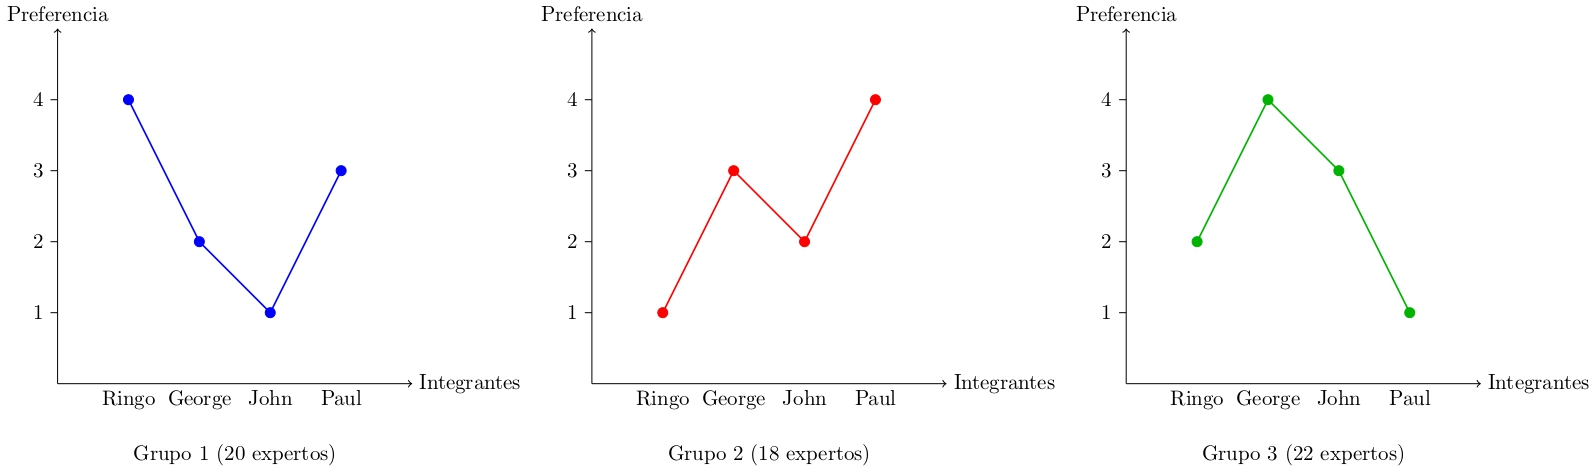
\includegraphics[keepaspectratio]{ecopol_beatles1.jpg}}

}

\caption{Preferencias ejercicio The Beatles}

\end{figure}%

\subsection{Modelo de Meltzer \& Richard}\label{2_2}

\begin{enumerate}
\def\labelenumi{\arabic{enumi})}
\setcounter{enumi}{5}
\tightlist
\item
  Suponga una sociedad conformada por \(n_{p}=530\) individuos pobre y
  \(n_{r}=123\) individuos ricos y que éstos tienen un ingreso de
  \(y_{p}=112\) y de \(y_{r}=150\), respectivamente. A partir de aquí
  suponga un impuesto a las ganancias del \(9\%\). Con esta información,
  responda:

  \begin{enumerate}
  \def\labelenumii{\roman{enumii})}
  \tightlist
  \item
    ¿Cuál es el ingreso directo de los pobres?
  \item
    Si se somete a votación por mayoría absoluta una nueva alícuota del
    \(12\%\) ¿Qué sucedería?
  \item
    ¿Existe desigualdad? ¿Por qué?
  \end{enumerate}
\end{enumerate}

\subsection{Pico Único y Cruce Único}\label{2_3}

\begin{enumerate}
\def\labelenumi{\arabic{enumi})}
\setcounter{enumi}{6}
\tightlist
\item
  De acuerdo a los siguiente gráficos de preferencias politicas
  determine:
\end{enumerate}

\begin{enumerate}
\def\labelenumi{\alph{enumi})}
\tightlist
\item
  ¿Son preferencias de pico único?
\item
  ¿Son preferencias de Cruce único?
\end{enumerate}

\newpage

\section{Unidad 3}\label{3}

\subsection{Modelo simple de no democracia}\label{3_1}

\begin{enumerate}
\def\labelenumi{\arabic{enumi})}
\setcounter{enumi}{7}
\tightlist
\item
  En 1810, la élite española concentraba el 80\% de la riqueza del
  Virreinato del Río de la Plata. Los criollos lograron organizarse, por
  lo que su poder para la revolución es alto (Estado de la Naturaleza
  H). La guerra revolucionaria y el costo en vidas asociado a ella
  destruiría el 30\% de los recursos disponibles. Determine cual es la
  resolución de este juego.
\end{enumerate}

\subsection{Modelo Democratización}\label{3_2}

\begin{enumerate}
\def\labelenumi{\arabic{enumi})}
\setcounter{enumi}{8}
\tightlist
\item
  En 1992, la élite afrikaaner representaba el 21\% de la población y
  concentraba el 90\% de los recursos de Sudáfrica. El African National
  Congress (ANC) logró, luego de mucho tiempo, organizarse de la mano de
  Nelson Mandela y reunir el poder de facto necesario para la revolución
  (Estado de la Naturaleza H). La revolución sería catastrófica:
  destruiría el 50\% de la riqueza. El umbral para la redistribución, de
  acuerdo con lo que está dispuesta a ceder la élite, es de 0.7,
  mientras que el umbral para la democratización es de 0.3. Determine
  cual es la resolución de este juego.
\end{enumerate}

\newpage

\section{Unidad 4}\label{4}




\end{document}
